
\documentclass{beamer}

\usepackage{amsmath}
\usepackage{amsfonts}
\usepackage{amssymb}

\newcommand\dx{\text{dx}}
\begin{document}
\title{Locking}
\author{Yngve Mardal Moe, Åshild Telle \& Roar Emaus}
\date{\today}
\frame{\titlepage}

\section{Intro}
\frame{
\frametitle{Linear elasticity}
\begin{itemize}
    \item Linear elasticity is a model of how solid objects deform
    \item Equation from Hook's Law (small deformations, isotropic media)
    \begin{itemize}
        \item $-2\mu\nabla \cdot \epsilon(u) + \lambda \nabla(\nabla\cdot u) = f$
    \end{itemize}
    \item $u$ is the deformation field we want to find
    \item $\lambda$ and $\mu$ are the material-dependent Lam\`e parameters
        \begin{itemize}
            \item Loosly said:
            \item $\lambda$ is tied to compressibility, larger means more incompressible
            \item $\mu$ is tied to stiffness, larger means harder to deform
        \end{itemize}
    \item $\epsilon$ is the symmetric gradient
\end{itemize}
}

\frame{
\frametitle{Simplest form}
\begin{itemize}
    \item Homogenous Dirichlet conditions
    \item Elasticity equation is:
        \begin{align*}
            -2\mu\nabla\cdot\epsilon(u) - \lambda\nabla\nabla\cdot u &= f \text{ in }\Omega,\\
            u &= 0 \text{ on } \partial\Omega\\
        \end{align*}
\end{itemize}
}

\frame{
\frametitle{Weak form}
\begin{align*}
    &\text{Multiply by test function and integrate:}&&\\
    &-2\mu\int_{\Omega} (\nabla\cdot\epsilon(u))\cdot v \dx 
    - \lambda\int_{\Omega}\nabla(\nabla\cdot u)\cdot v \dx &&= \int_{\Omega}f\cdot v \dx\\
    &\text{ Integration by parts: }\\
    &2\mu\int_{\Omega}\epsilon(u)\cdot \nabla v \dx 
    + \lambda\int_{\Omega}(\nabla\cdot u)(\nabla\cdot v) \dx &&= \int_{\Omega}f\cdot v \dx\\
    &A:B = A:B_S \text{ if } A = A^T\text{:}\\
    &2\mu\int_{\Omega}\epsilon(u)\cdot \epsilon(v) \dx 
    + \lambda\int_{\Omega}(\nabla\cdot u)(\nabla\cdot v) \dx &&= \int_{\Omega}f\cdot v \dx\\
\end{align*}
}

\frame{
\frametitle{Weak form cont.}
Find $u \in H_0^1$ such that
\begin{align*}
    a(u, v) &= f(v), \forall v\in H_0^1&&\\
    \text{ where} \\
    a(u,v) &= 2\mu(\epsilon(u), \epsilon(v)) + \lambda(\nabla\cdot u, \nabla\cdot v),\\
    f(v) &= (f,v)
\end{align*}
}

\frame{
\frametitle{Locking}
\begin{itemize}
    \item Locking arises from numerical errors when $\lambda \gg \mu$
    \item Difficulty in optimizing both $\nabla (u - u_h)$ and $\nabla\cdot (u - u_h) = 0$ at the same time
\end{itemize}
}

\frame{
\frametitle{Locking from an optimisation standpoint}
Solving the elasticity equation with the finite element method is equivalent to solving
\begin{align}
	\min_{u_h \in U_h} \|u - u_h\|_a^2 = \min_{u_h \in U_h} \|\nabla (u - u_h)\|_{L^2}^2 + \lambda \| \nabla \cdot (u - u_h) \|_{L^2}^2.
\end{align}
To understand locking, we let \(\lambda \to \infty\) and obtain
\begin{align}
	\min_{u_h \in U_h} & \|\nabla (u - u_h)\|_{L^2}^2 \nonumber \\
	\text{s.t.}~ & (\nabla \cdot (u - u_h), v_h) = 0 \qquad \text{for all}~v_h \in U_h.
\end{align}
}

%\frame{
%\frametitle{Helmholz decomposition theorem}
%\begin{itemize}
%    \item Any field $L^2$ or $H^1$ can be decomposed into sum of a gradient and a curl
%    \item $u = \nabla\phi + \nabla\times\psi$
%    \item $\phi$, irrotational
%    \item $\psi$, solenoidal
%\end{itemize}
%}

\frame{
\frametitle{Medicinal pressure}
\begin{itemize}
    \item Introduce solid pressure $p$
    \item $p = \lambda\nabla\cdot u$
\end{itemize}
New equation is then:
\begin{align*}
    -\mu\Delta u - \nabla p &= f,\\
    \nabla\cdot u - \frac{1}{\lambda}p &= 0\\
\end{align*}

As material becomes incompressible, $\lambda \rightarrow \infty$, the equations becomes
the Stokes problem as $\frac{1}{\lambda} \rightarrow 0$
}

\frame{
\frametitle{Weak form}
Find $u \in H^1_0$ and $p \in L^2$ such that
\begin{align*}
    a(u,v) + b(p,v) &= f &&\forall v \in H^1\\
    b(q, u) - c(p, q) &= 0 &&\forall q \in \mathbb{R}\\
\end{align*}
where
\begin{align*}
    a(u,v) &= (\epsilon(u), \epsilon(v))\\
    b(p,v) &= (p, \nabla\cdot v)\\
    c(p,q) &= \frac{1}{\lambda}(p\cdot q)\\
\end{align*}
}

\frame{
\frametitle{Saddle point interpretation of the two-field formulation}
The above equation is equivalent to solving the sadle point problem
\begin{align*}
	\max_{p \in Q_h} \min_{u \in V_h} a(u, u) + b(p, u) - \lambda^{-1} (p, p),
\end{align*}
where \(\lambda^{-1}\) works as a regulariser which means that we can circumvent the inf-sup condition.
}

\frame{
\frametitle{Deformation domains}
\begin{figure}
    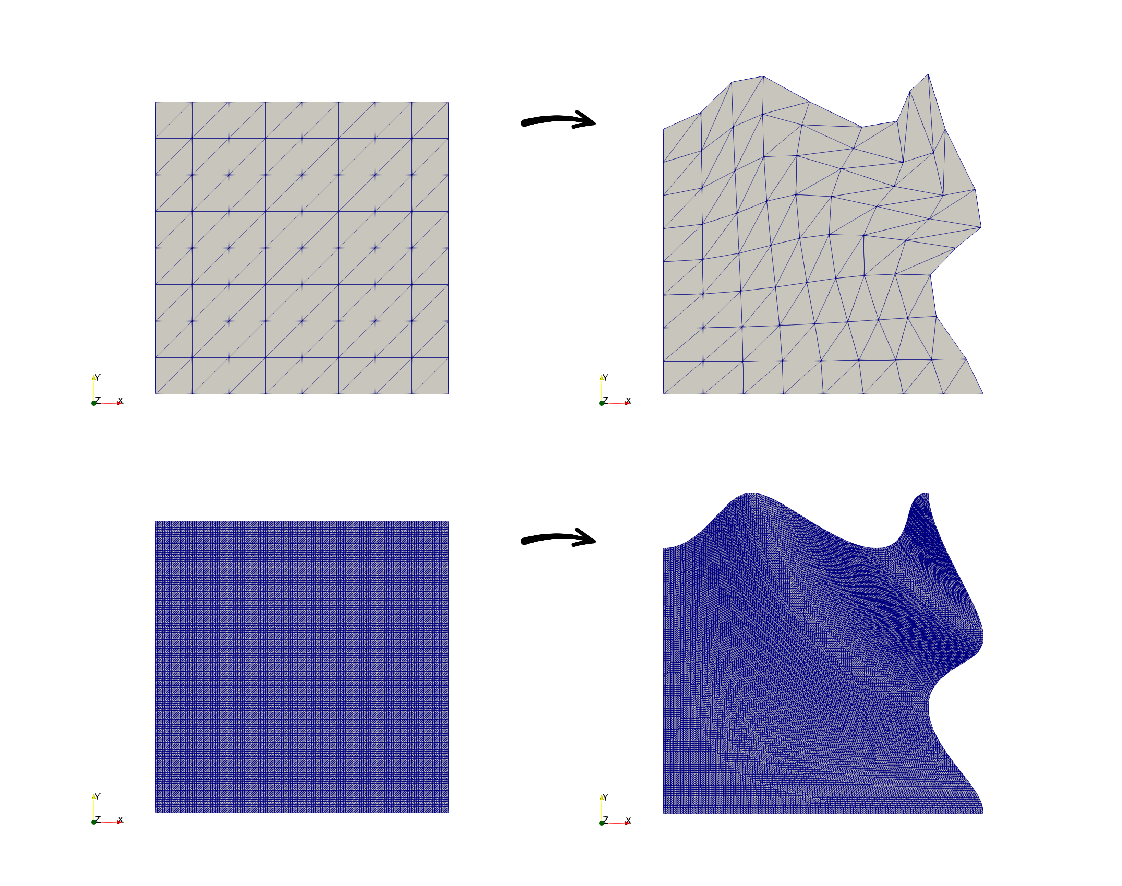
\includegraphics[width=1.0\textwidth]{plots/deformation_domains.pdf}
\end{figure}
}

\frame{
\frametitle{Deformation domains}
\begin{figure}
    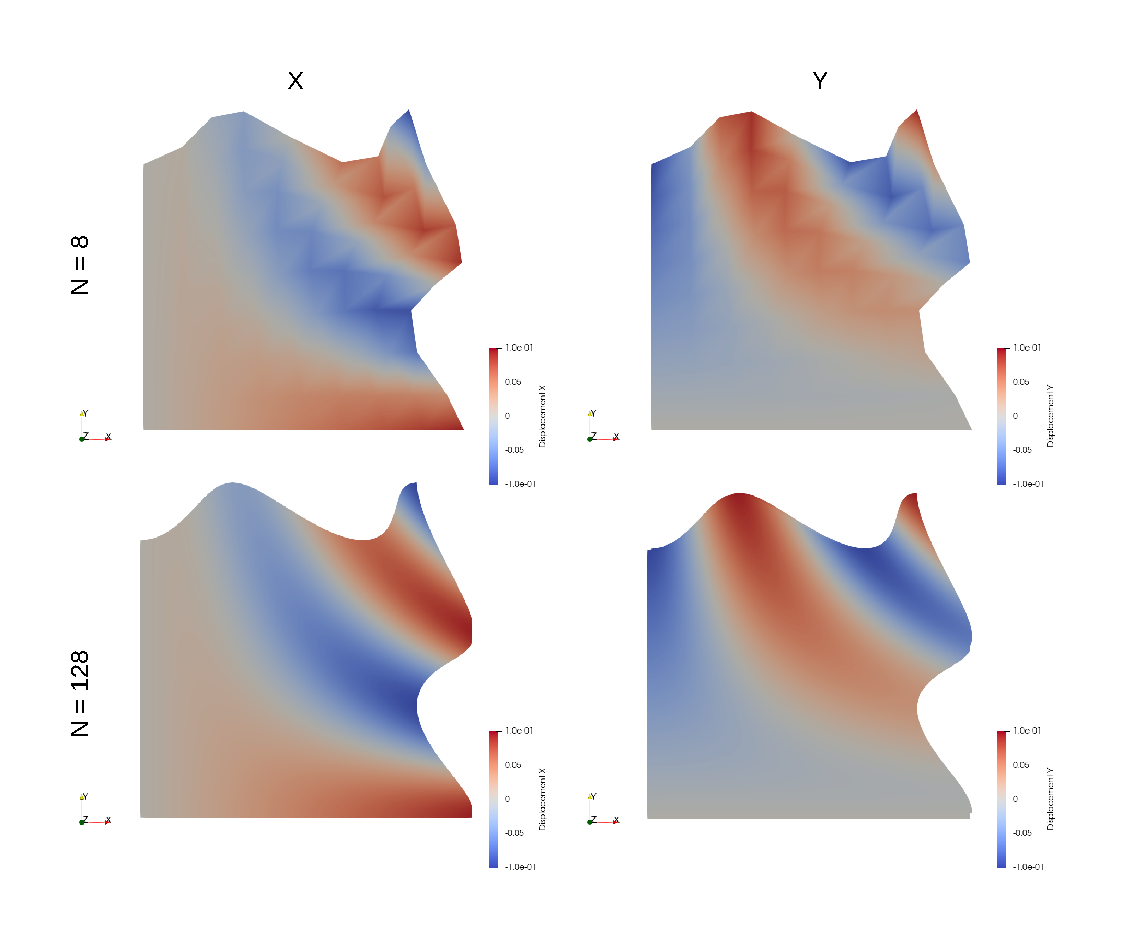
\includegraphics[width=1.0\textwidth]{plots/disp_xy.pdf}
\end{figure}
}

\frame{
\frametitle{Relative Error CG-1}
\begin{figure}
    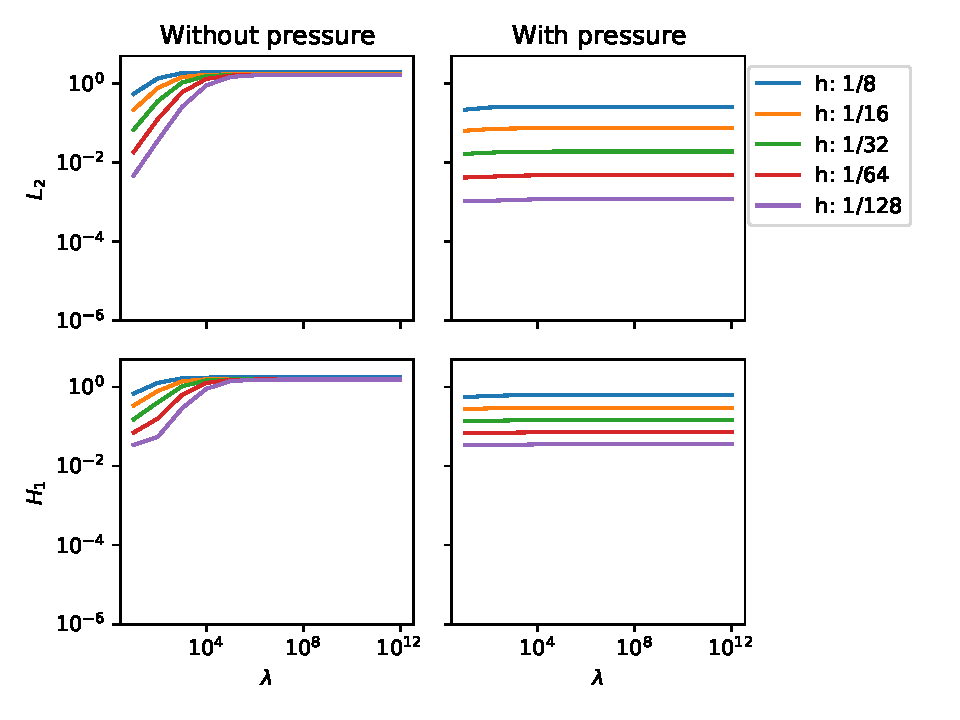
\includegraphics[width=1.0\textwidth]{plots/errors_norms_schemes_order_1.pdf}
\end{figure}
}

\frame{
\frametitle{Relative Error CG-2}
\begin{figure}
    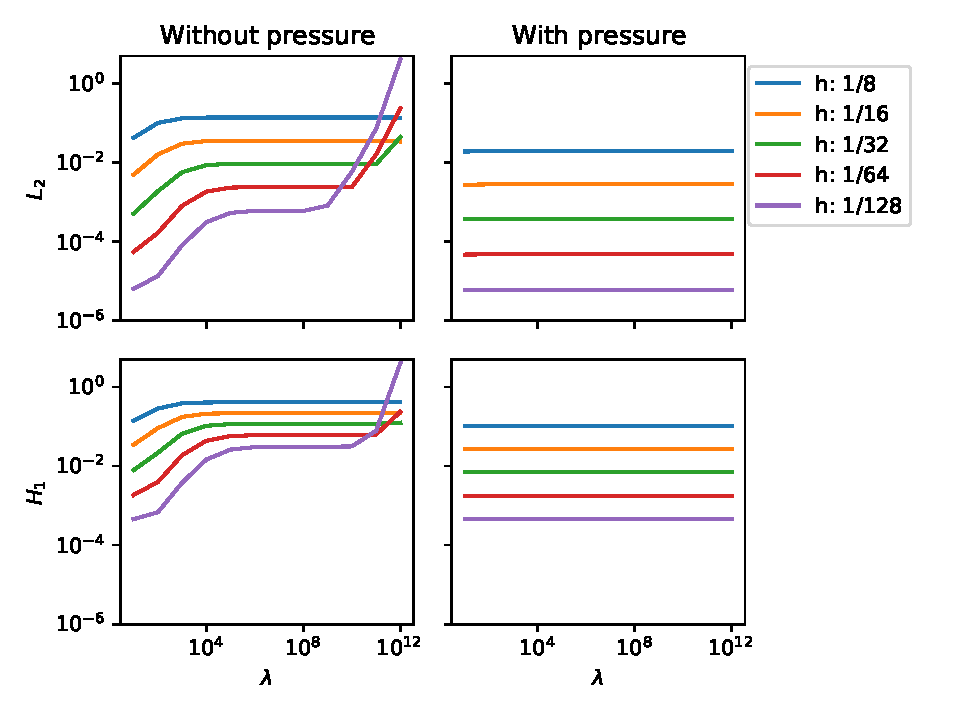
\includegraphics[width=1.0\textwidth]{plots/errors_norms_schemes_order_2.pdf}
\end{figure}
}

\frame{
\frametitle{Spatial plot of u, $\lambda = 10$ without solid pressure}
\begin{figure}
    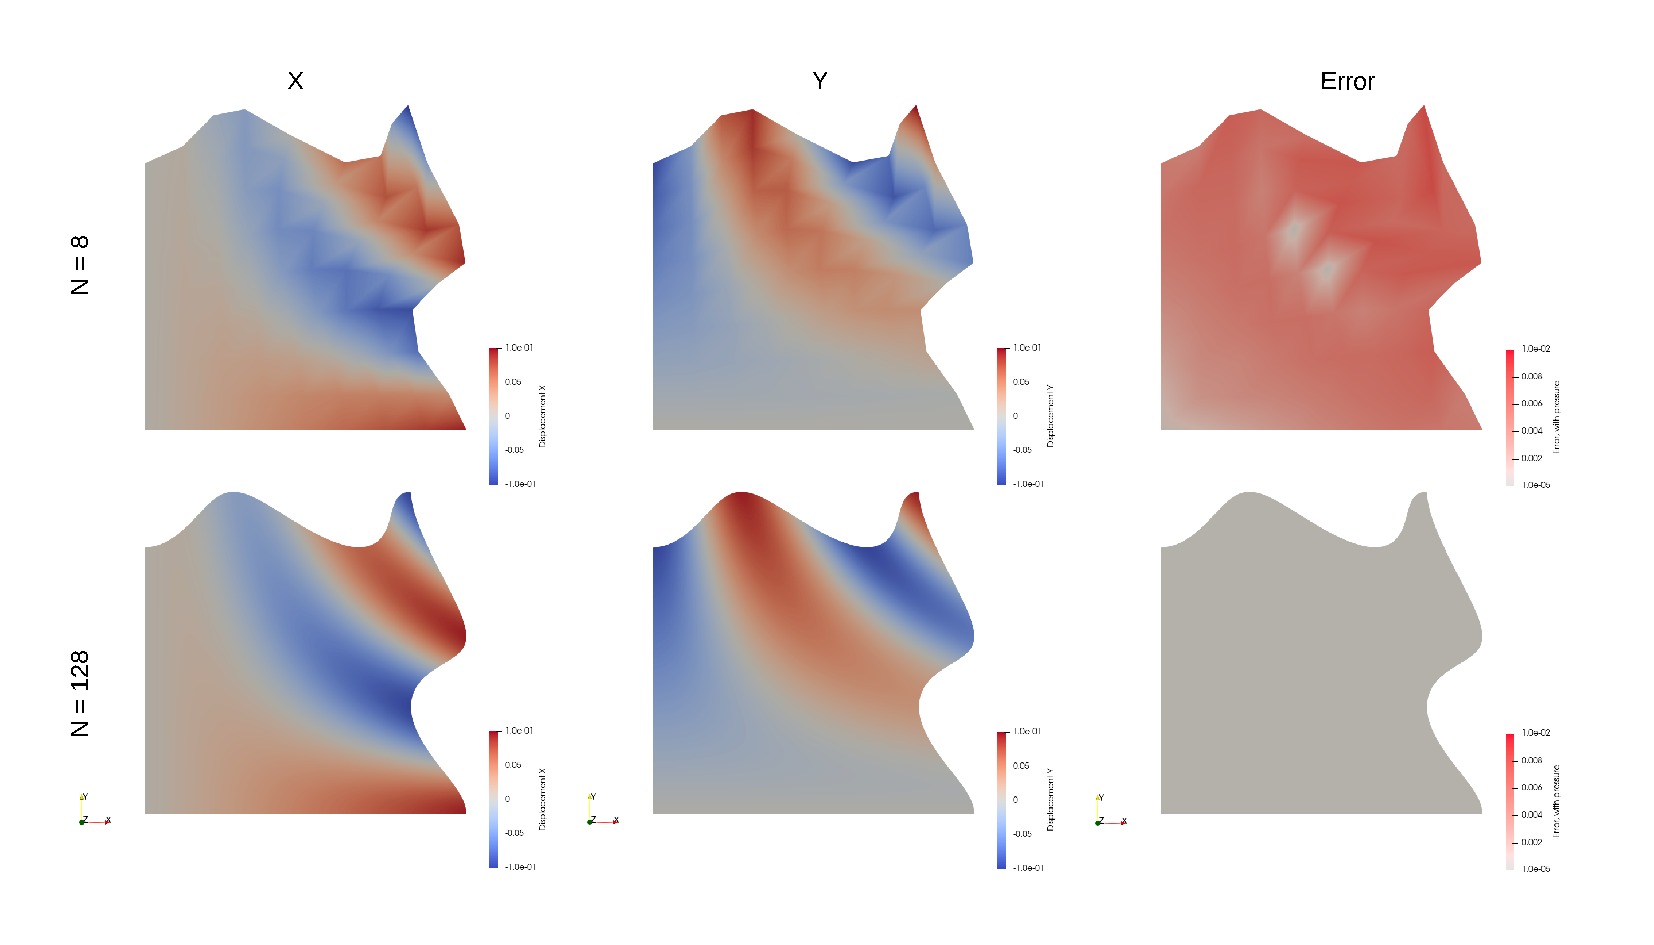
\includegraphics[width=1.0\textwidth]{plots/lambda_10_without.pdf}
\end{figure}
}

\frame{
\frametitle{Spatial plot of u, $\lambda = 10$ with solid pressure}
\begin{figure}
    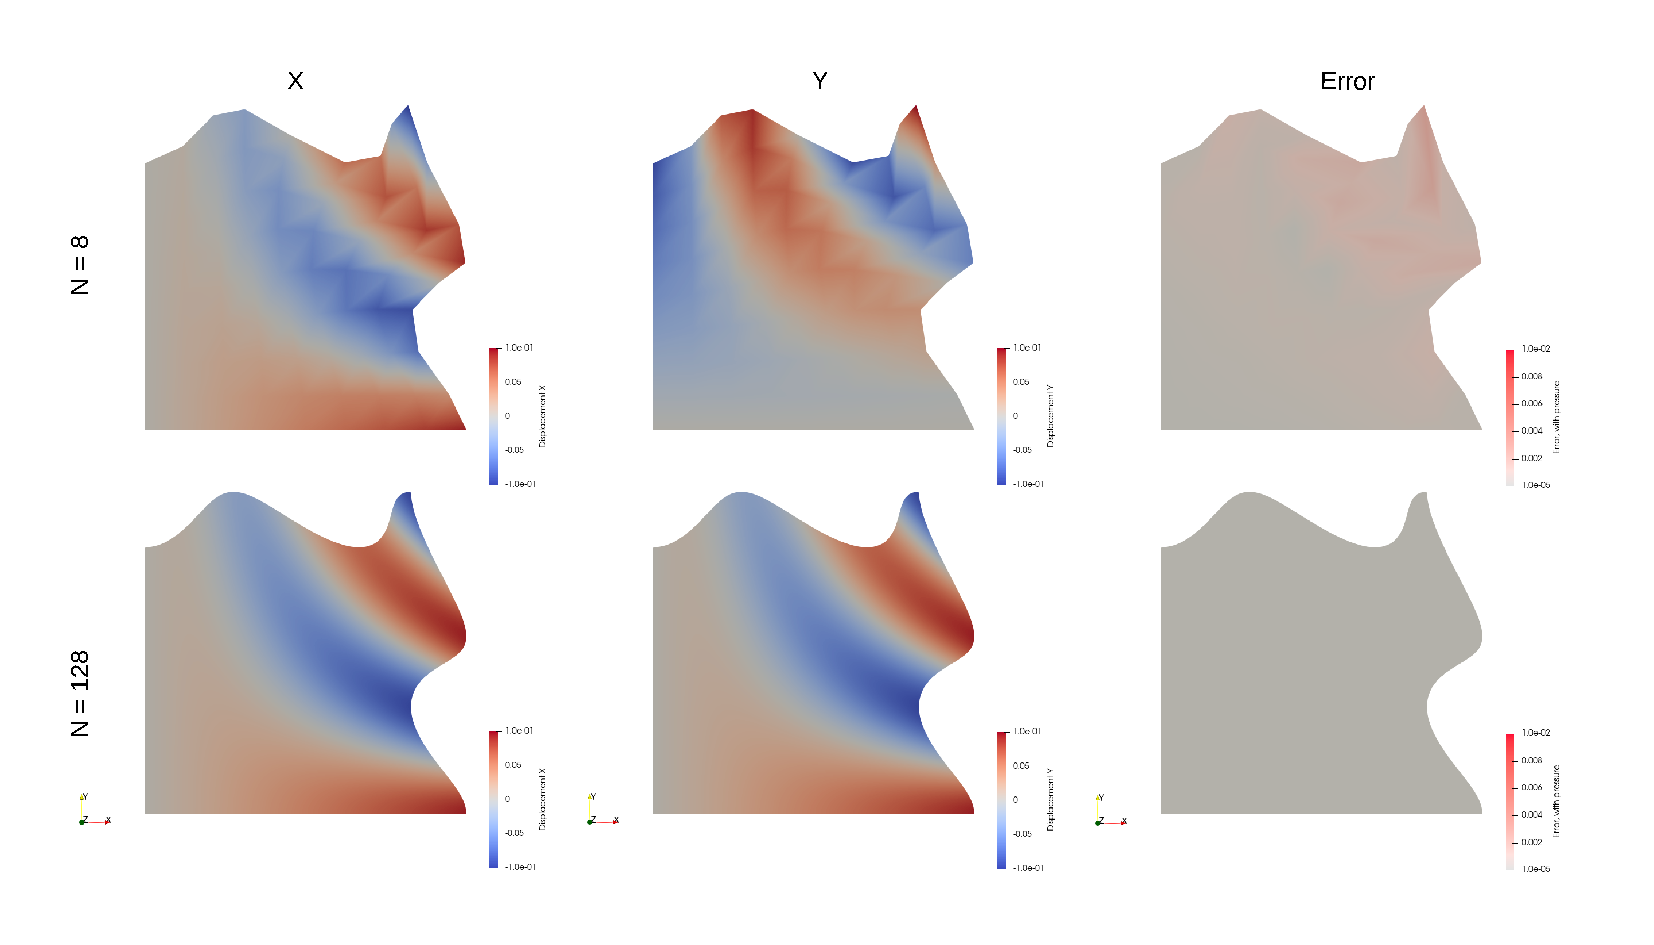
\includegraphics[width=1.0\textwidth]{plots/lambda_10_with.pdf}
\end{figure}
}

\frame{
\frametitle{Spatial plot of u, $\lambda = 10^{12}$, without solid pressure}
\begin{figure}
    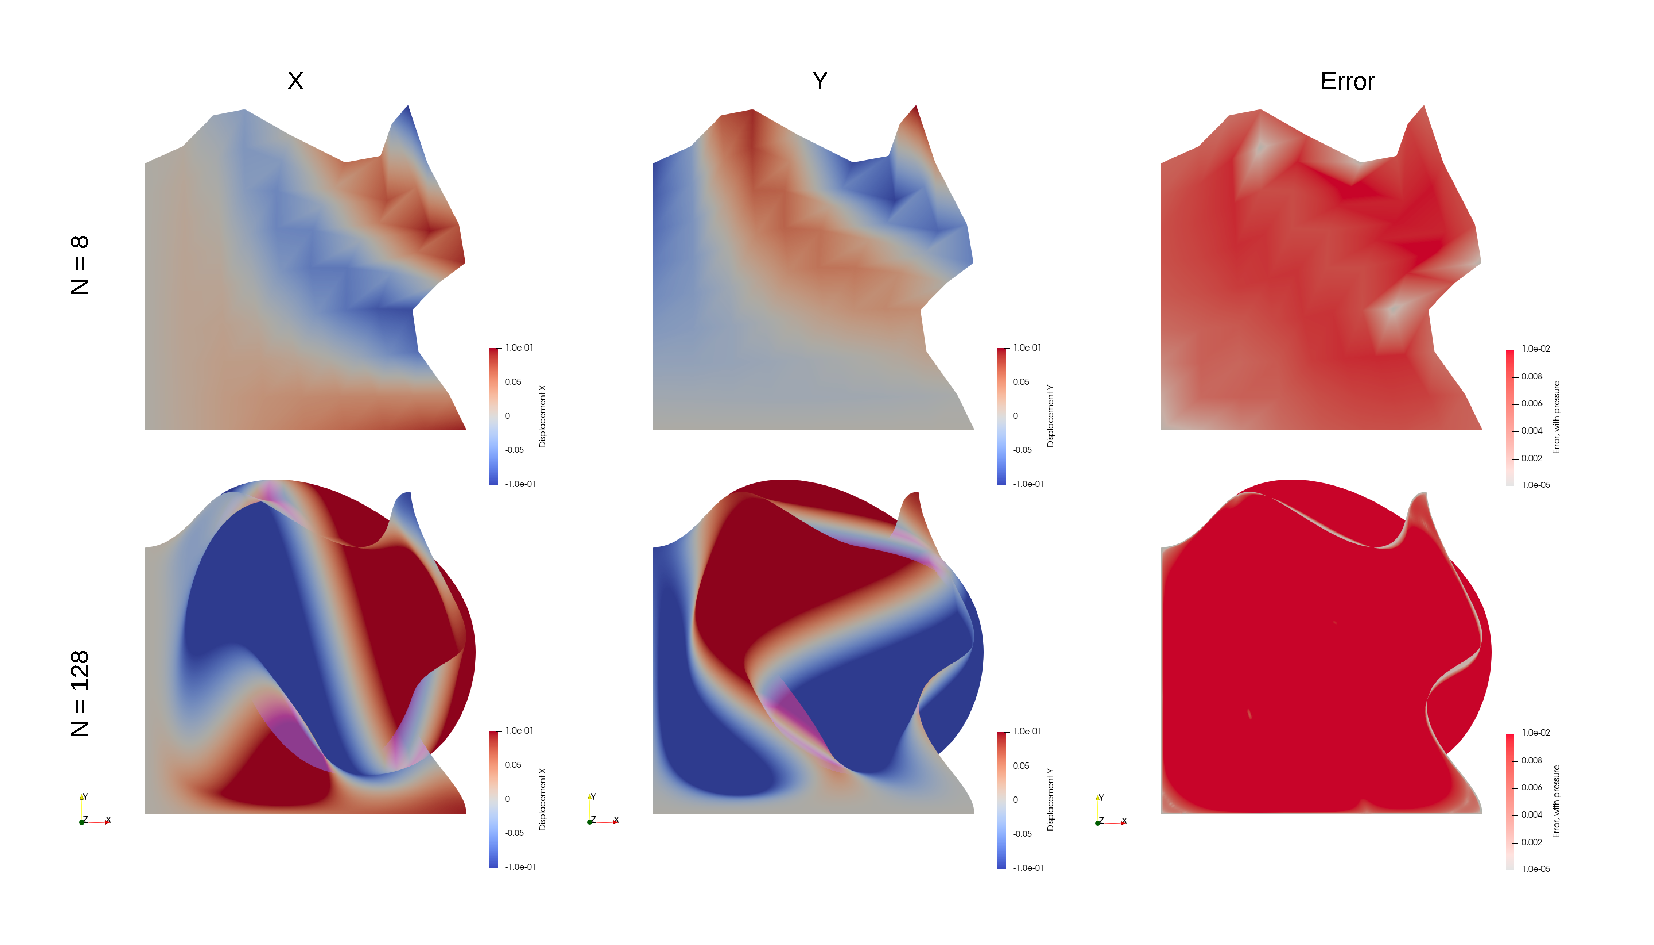
\includegraphics[width=1.0\textwidth]{plots/lambda_1e12_without.pdf}
\end{figure}
}

\frame{
\frametitle{Spatial plot of u, $\lambda = 10^{12}$, with solid pressure}
\begin{figure}
    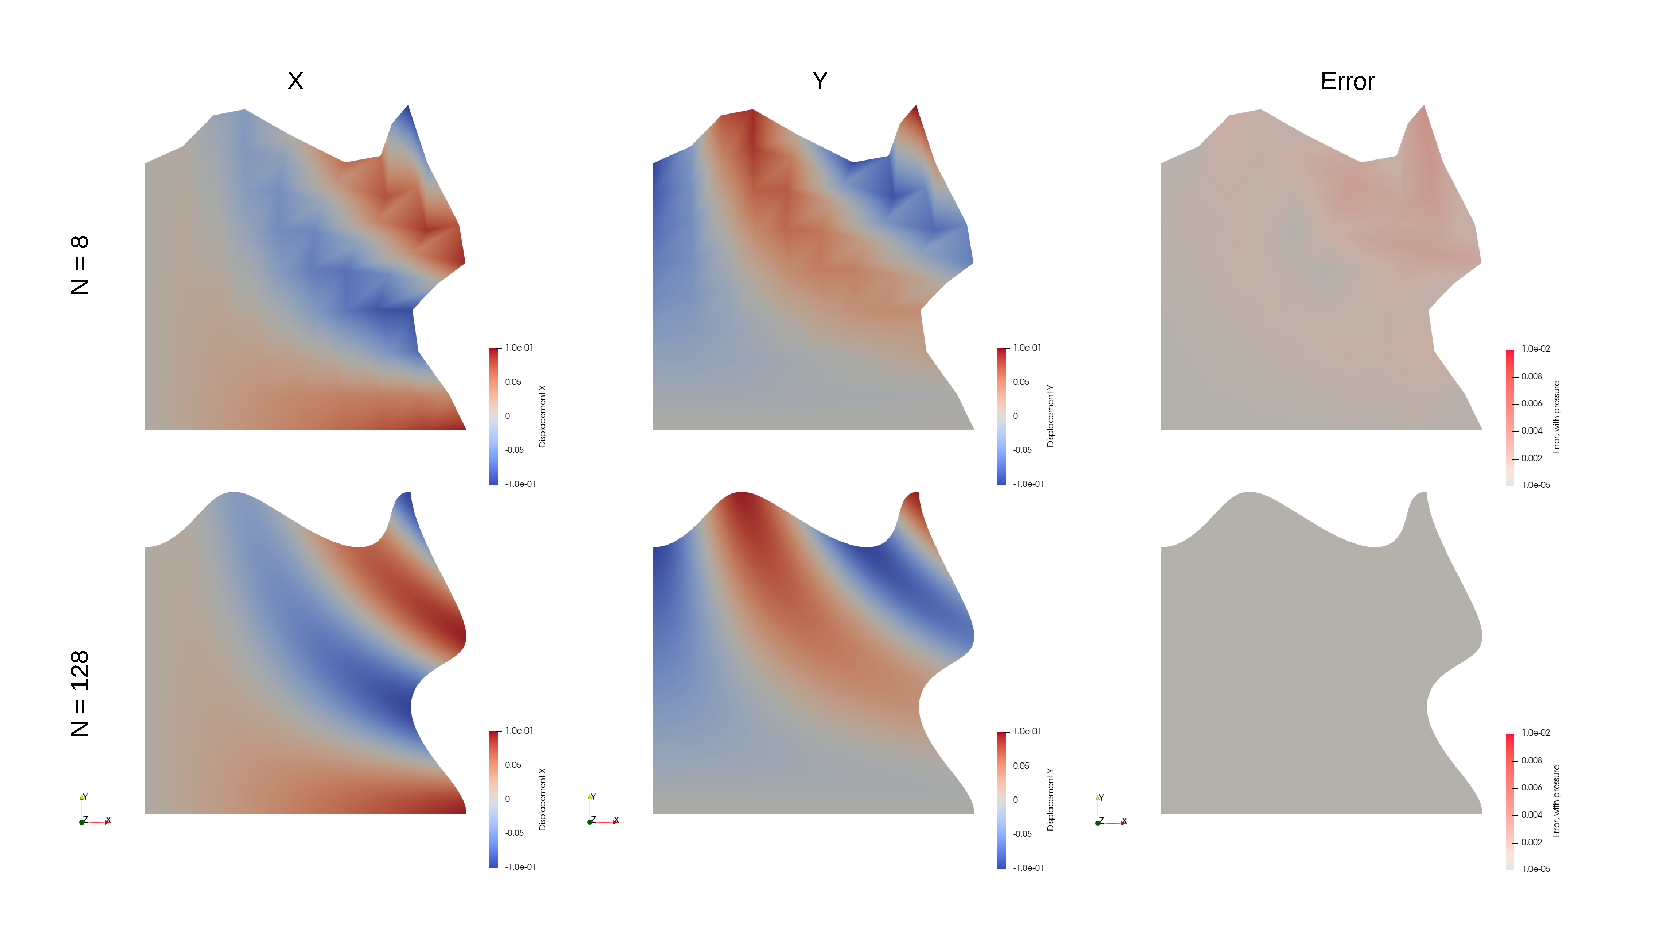
\includegraphics[width=1.0\textwidth]{plots/lambda_1e12_with.pdf}
\end{figure}
}

\end{document}
